%%%%%%%%%%%%%%%%%%%%%%%%%%%%%%%%%%%%%%%%%%%%%%%%%%%%%%%%%%%%%%%%%%%%%%%%%%%%%%%%%%
\begin{frame}[fragile]\frametitle{}
\begin{center}
{\Large Framework}
\end{center}
\end{frame}



%%%%%%%%%%%%%%%%%%%%%%%%%%%%%%%%%%%%%%%%%%%%%%%%%%%%%%%%%%%
\begin{frame}[fragile]\frametitle{LangChain: Build Apps with LLMs}

\begin{itemize}
\item LangChain: Open-source framework for building applications with LLMs.
\item Capabilities: Enhances LLMs with prompt templates and integration of different APIs and external databases.
\item Application Examples: Building chatbots, Q\&A platforms, and real-time natural language understanding applications.
\item Data Discovery: Index text data into a vector database, partition into chunks, encode chunks into embeddings, and search for data using cosine similarity.
\item Prompt Engineering: Insert users' questions within prompt templates, provide context through examples, and create prompts with multiple (prompt, answer) pairs if needed.
\item Tools and Memory: LLM can utilize tools like Google Search, Python REPL, etc., and remember previous discussions through memory.
\item Challenges: Juggling questions, prompt templates, data search, tools, plan of action, and memory for constructing meaningful prompts.
\item LangChain Benefits: Powerful LLMops tool with an abstracted interface, API connection to public LLMs, integration with various tools and vector databases.
\item Visual Summary: Flowchart depicting the entire process.
\end{itemize}

{\tiny (Ref: Overview of Large Language Models - Aman AI)}

\end{frame}

%%%%%%%%%%%%%%%%%%%%%%%%%%%%%%%%%%%%%%%%%%%%%%%%%%%%%%%%%%%
\begin{frame}[fragile]\frametitle{LangChain: Build Apps with LLMs}

		\begin{center}
		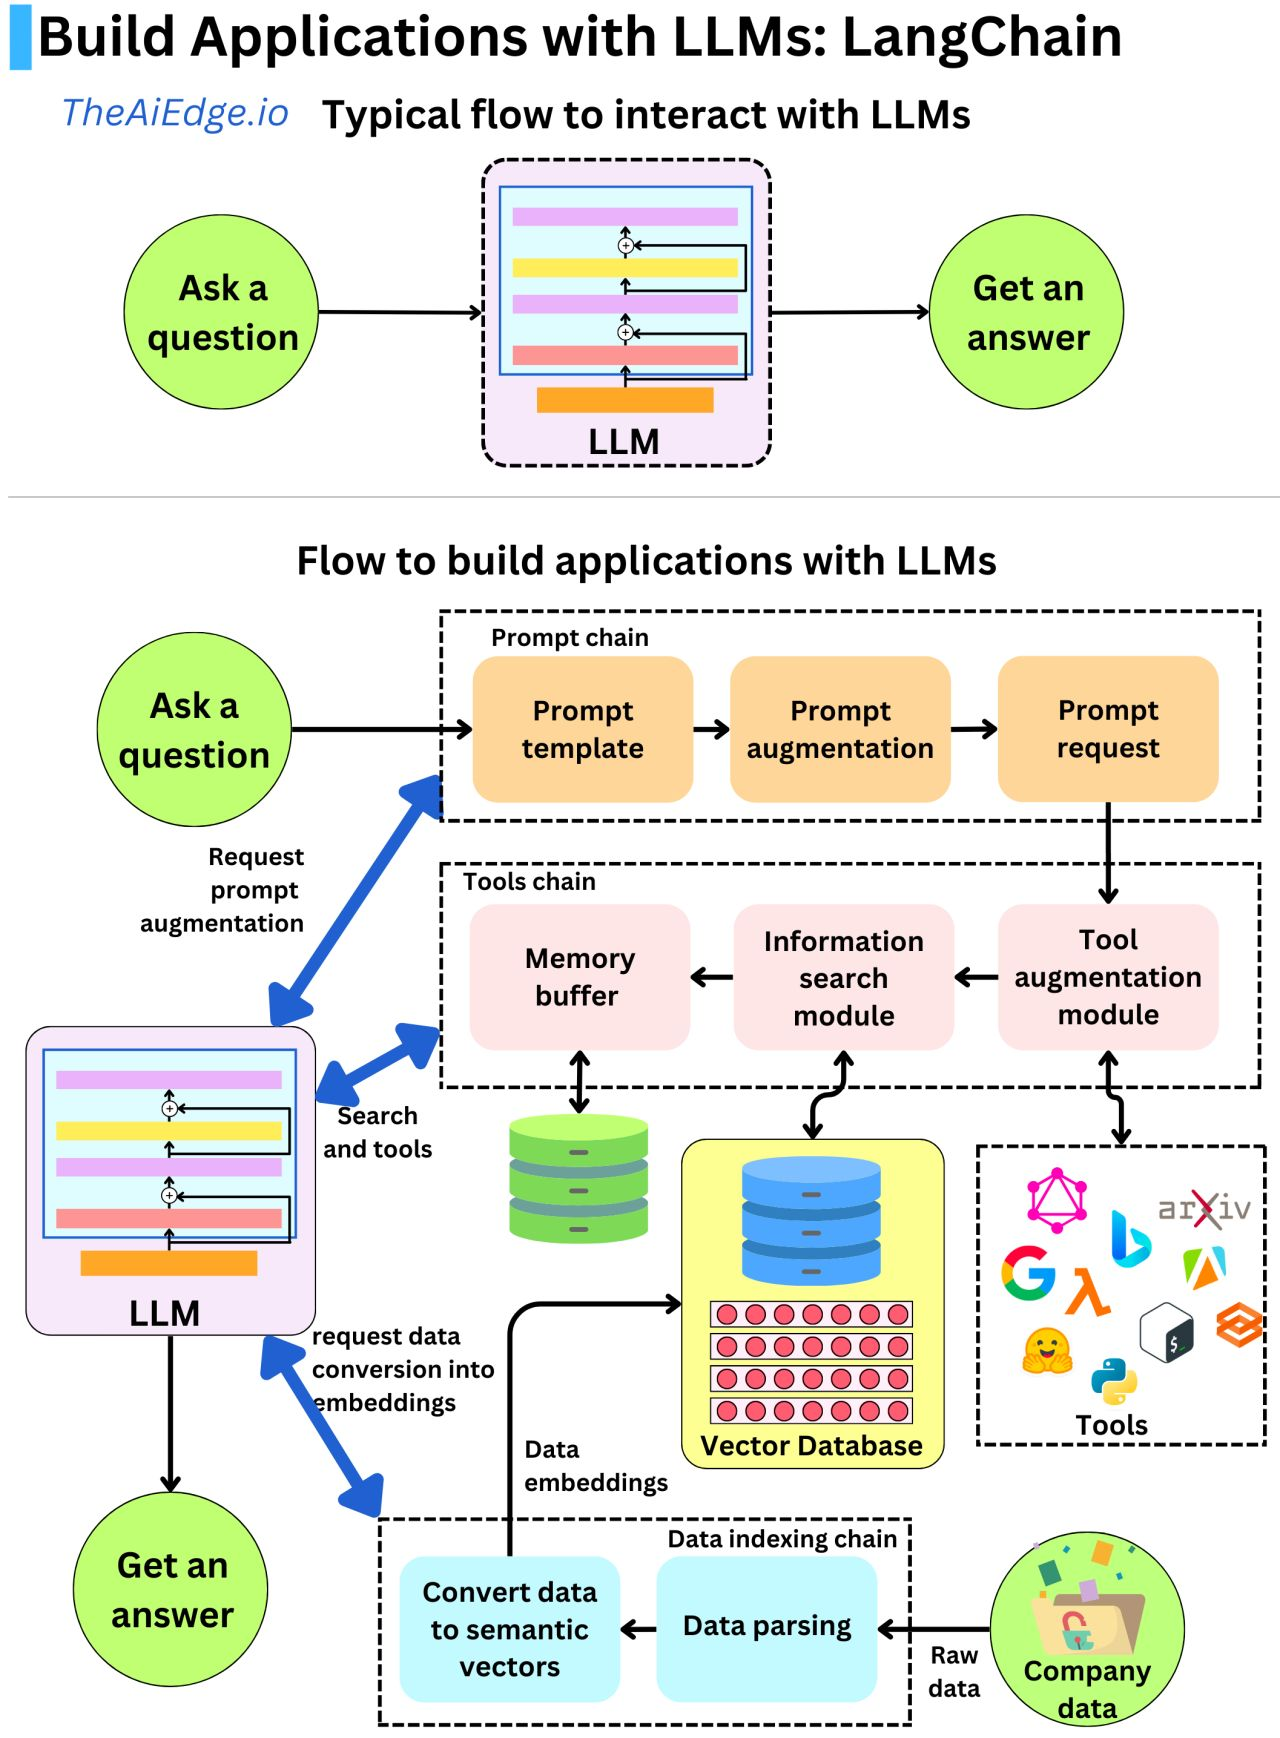
\includegraphics[width=0.8\linewidth,keepaspectratio]{chatgpt48}
		\end{center}
		
{\tiny (Ref: Overview of Large Language Models - Aman AI)}

\end{frame}


%%%%%%%%%%%%%%%%%%%%%%%%%%%%%%%%%%%%%%%%%%%%%%%%%%%%%%%%%%%%%%%%%%%%%%%%%%%%%%%%%%
\begin{frame}[fragile]\frametitle{LangChain Components}

\begin{center}
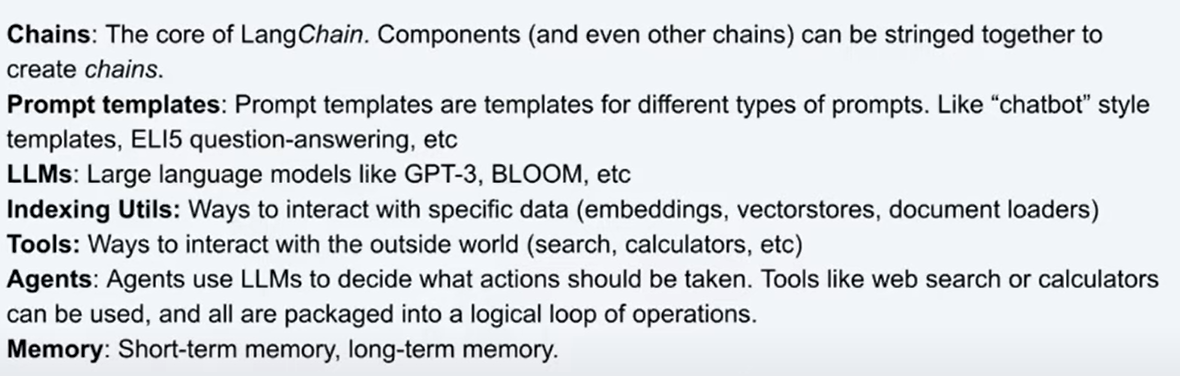
\includegraphics[width=\linewidth,keepaspectratio]{langchain1}
\end{center}	  

{\tiny (Ref: Building the Future with LLMs, LangChain, \& Pinecone)}
\end{frame}

%%%%%%%%%%%%%%%%%%%%%%%%%%%%%%%%%%%%%%%%%%%%%%%%%%%%%%%%%%%%%%%%%%%%%%%%%%%%%%%%%%
\begin{frame}[fragile]\frametitle{}
\begin{center}
{\Large Data Loaders}
\end{center}
\end{frame}

%%%%%%%%%%%%%%%%%%%%%%%%%%%%%%%%%%%%%%%%%%%%%%%%%%%%%%%%%%%%%%%%%%%%%%%%%%%%%%%%%%
\begin{frame}[fragile]\frametitle{LangChain Data Loaders}

There are a lot of document loaders: File Loader, Directory Loader, Notion, ReadTheDocs, HTML, PDF, PowerPoint, Email, GoogleDrive, Obsidian, Roam, EverNote, YouTube, Hacker News, GitBook, S3 File, S3 Directory, GCS File, GCS Directory, Web Base, IMSDb, AZLyrics, College Confidential, Gutenberg, Airbyte Json, CoNLL-U, iFixit, Notebook, Copypaste, CSV, Facebook Chat, Image, Markdown, SRT, Telegram, URL, Word Document, Blackboard

Langchain will chunk the documents and then index its vectors.

\begin{lstlisting}
from langchain.document_loaders import TextLoader
loader = TextLoader('state_of_the_union.txt')
from langchain.indexes import VectorstoreIndexCreator
index = VectorstoreIndexCreator().from_loaders([loader])
query = "What did the president say about Ketanji Brown Jackson"
index.query(query)
\end{lstlisting}	  

\end{frame}


%%%%%%%%%%%%%%%%%%%%%%%%%%%%%%%%%%%%%%%%%%%%%%%%%%%%%%%%%%%%%%%%%%%%%%%%%%%%%%%%%%
\begin{frame}[fragile]\frametitle{}
\begin{center}
{\Large Memory}
\end{center}
\end{frame}

%%%%%%%%%%%%%%%%%%%%%%%%%%%%%%%%%%%%%%%%%%%%%%%%%%%%%%%%%%%%%%%%%%%%%%%%%%%%%%%%%%
\begin{frame}[fragile]
\frametitle{Need}

\begin{itemize}
    \item LangChain's ConversationChain has a simple type of memory.
    \item The memory remembers all previous inputs/outputs and adds them to the context passed.
    \item This memory can be considered a type of short-term memory.
    \item Example: How to use ConversationChain with short-term memory.
    \item It can remember the initial messages even after 3 questions.
\end{itemize}

\begin{lstlisting}
from langchain import OpenAI, ConversationChain

llm = OpenAI(model_name="text-davinci-003", temperature=0)
conversation = ConversationChain(llm=llm, verbose=True)

output = conversation.predict(input="Hi there!")

print(output)

> Entering new ConversationChain chain...

Prompt after formatting:

The following is a friendly conversation between a human and an AI. The AI is talkative and provides lots of specific details from its context. If the AI does not know the answer to a question, it truthfully says it does not know.

Current conversation:

Human: Hi there!
AI:

> Finished chain.

Hi there! It's nice to meet you. How can I help you today?
\end{lstlisting}

\end{frame}

%%%%%%%%%%%%%%%%%%%%%%%%%%%%%%%%%%%%%%%%%%%%%%%%%%%%%%%%%%%%%%%%%%%%%%%%%%%%%%%%%%
\begin{frame}[fragile]
\frametitle{ConversationBufferMemory}

\begin{itemize}
    \item ConversationChain uses the ConversationBufferMemory class by default to store a history of messages.
    \item This memory saves previous conversations in the form of variables.
    \item The class accepts the return\_messages argument, which is useful for dealing with chat models.
\end{itemize}

\begin{lstlisting}
from langchain.memory import ConversationBufferMemory

memory = ConversationBufferMemory(return_messages=True)
memory.save_context({"input": "hi there!"}, {"output": "Hi there! It's nice to meet you. How can I help you today?"})

print( memory.load_memory_variables({}) )

>>{'history': [HumanMessage(content='hi there!', additional_kwargs={}, example=False),
  AIMessage(content="Hi there! It's nice to meet you. How can I help you today?", additional_kwargs={}, example=False)]}
\end{lstlisting}

\end{frame}

%%%%%%%%%%%%%%%%%%%%%%%%%%%%%%%%%%%%%%%%%%%%%%%%%%%%%%%%%%%%%%%%%%%%%%%%%%%%%%%%%%
\begin{frame}[fragile]
\frametitle{ConversationBufferMemory}

\begin{itemize}
    \item This memory implementation stores the entire conversation history as a single string.
    \item Advantages:
    \begin{itemize}
        \item Maintains a complete record of the conversation.
        \item Straightforward to implement and use.
    \end{itemize}
    \item Disadvantages:
    \begin{itemize}
        \item Less efficient as the conversation grows longer.
        \item May lead to excessive repetition if the conversation history is too long for the model's token limit.
    \end{itemize}
\end{itemize}

\end{frame}

%%%%%%%%%%%%%%%%%%%%%%%%%%%%%%%%%%%%%%%%%%%%%%%%%%%%%%%%%%%%%%%%%%%%%%%%%%%%%%%%%%
\begin{frame}[fragile]
\frametitle{ConversationBufferMemory (Contd.)}

\begin{itemize}
    \item If the model's token limit is surpassed, the buffer gets truncated to fit within the limit.
    \item Older interactions may be removed from the buffer to accommodate newer ones.
    \item This truncation may cause the conversation context to lose some information.
    \item To avoid surpassing the token limit:
    \begin{itemize}
        \item Monitor the token count in the buffer.
        \item Manage the conversation accordingly, e.g., shorten input texts or remove less relevant parts.
    \end{itemize}
\end{itemize}

\end{frame}

%%%%%%%%%%%%%%%%%%%%%%%%%%%%%%%%%%%%%%%%%%%%%%%%%%%%%%%%%%%%%%%%%%%%%%%%%%%%%%%%%%
\begin{frame}[fragile]
\frametitle{ConversationBufferWindowMemory}

\begin{itemize}
    \item This class limits memory size by keeping a list of the most recent K interactions.
    \item Maintains a sliding window of recent interactions to prevent the buffer from growing too large.
    \item Advantages:
    \begin{itemize}
        \item Stores a fixed number of recent messages, making it more efficient than ConversationBufferMemory.
        \item Reduces the risk of exceeding the model's token limit.
    \end{itemize}
\end{itemize}

\end{frame}

%%%%%%%%%%%%%%%%%%%%%%%%%%%%%%%%%%%%%%%%%%%%%%%%%%%%%%%%%%%%%%%%%%%%%%%%%%%%%%%%%%
\begin{frame}[fragile]
\frametitle{ConversationBufferWindowMemory (Contd.)}

\begin{itemize}
    \item Disadvantage:
    \begin{itemize}
        \item Does not maintain the complete conversation history.
        \item Chatbot might lose context if essential information falls outside the fixed window of messages.
    \end{itemize}
    \item Possible to retrieve specific interactions from ConversationBufferWindowMemory.
\end{itemize}

\end{frame}

%%%%%%%%%%%%%%%%%%%%%%%%%%%%%%%%%%%%%%%%%%%%%%%%%%%%%%%%%%%%%%%%%%%%%%%%%%%%%%%%%%
\begin{frame}[fragile]
\frametitle{ConversationSummaryMemory}
ConversationSummaryBufferMemory is a memory management strategy that combines the ideas of keeping a buffer of recent interactions in memory and compiling old interactions into a summary. It extracts key information from previous interactions and condenses it into a shorter, more manageable format. 
\textbf{Advantages:}
\begin{itemize}
    \item Condensing conversation information.
    \item Reducing the number of tokens required to store the conversation history.
    \item Flexibility in returning history as a list of messages or a plain text summary.
    \item Direct summary prediction with \texttt{predict\_new\_summary} method.
    \item Provides more control over the summarization process.
\end{itemize}

\textbf{Disadvantages:}
\begin{itemize}
    \item Loss of information in the summary.
    \item Possible omission of important details from the conversation.
    \item Increased complexity compared to simpler memory types like ConversationBufferMemory.
\end{itemize}

\end{frame}


%%%%%%%%%%%%%%%%%%%%%%%%%%%%%%%%%%%%%%%%%%%%%%%%%%%%%%%%%%%
\begin{frame}[fragile]\frametitle{Memory}

\begin{itemize}
\item OpenAI's API as the most powerful LLM API today
\item Non-stateful nature of the API requires passing back necessary context for each request
\item Light weight options for storing message history (Python list, text file) but not scalable
\item Spin up a vector database for embeddings, but requires additional work
\item Langchain's memory module for automatic message history storage
\item Plug and play access to multiple data stores
\item Reduction of friction in creating chatbots, for example
\item Langchain's support for 10 different database integrations
\item Increasing options outside Langchain for managing chat history and truncation
\item Truncation process: narrowing down message history to fit within context window
\item Different approaches to truncation with no perfect solution
\item Importance of embeddings and memory in Langchain for managing chat history.
\end{itemize}

{\tiny (Ref: What is Langchain and why should I care as a developer? - Logan Kilpatrick)}

\end{frame}

%%%%%%%%%%%%%%%%%%%%%%%%%%%%%%%%%%%%%%%%%%%%%%%%%%%%%%%%%%%%%%%%%%%%%%%%%%%%%%%%%%
\begin{frame}[fragile]\frametitle{LangChain Memory}

Keeps chat history in memory. You can also summarize the chat history.

\begin{lstlisting}
from langchain.llms import OpenAI
from langchain.prompts import PromptTemplate
from langchain.chains import ConversationChain
from langchain.memory import ConversationBufferWindowMemory, CombinedMemory, ConversationSummaryMemory


conv_memory = ConversationBufferWindowMemory(
    memory_key="chat_history_lines",
    input_key="input",
    k=1
)

summary_memory = ConversationSummaryMemory(llm=OpenAI(), input_key="input")
# Combined
memory = CombinedMemory(memories=[conv_memory, summary_memory])
_DEFAULT_TEMPLATE = """The following is a friendly conversation between a human and an AI. The AI is talkative and provides lots of specific details from its context. If the AI does not know the answer to a question, it truthfully says it does not know.

\end{lstlisting}	  

\end{frame}


%%%%%%%%%%%%%%%%%%%%%%%%%%%%%%%%%%%%%%%%%%%%%%%%%%%%%%%%%%%%%%%%%%%%%%%%%%%%%%%%%%
\begin{frame}[fragile]\frametitle{LangChain Memory}


\begin{lstlisting}
Summary of conversation:
{history}
Current conversation:
{chat_history_lines}
Human: {input}
AI:"""
PROMPT = PromptTemplate(
    input_variables=["history", "input", "chat_history_lines"], template=_DEFAULT_TEMPLATE
)
llm = OpenAI(temperature=0)
conversation = ConversationChain(
    llm=llm, 
    verbose=True, 
    memory=memory,
    prompt=PROMPT
)

conversation.run("Hi!")
conversation.run("Can you tell me a joke?")
conversation.run("Can you tell me a similar joke?")
\end{lstlisting}	  

\end{frame}


%%%%%%%%%%%%%%%%%%%%%%%%%%%%%%%%%%%%%%%%%%%%%%%%%%%%%%%%%%%%%%%%%%%%%%%%%%%%%%%%%%
\begin{frame}[fragile]
\frametitle{Recap and Strategies}

\textbf{Strategies to Manage Token Limit:}
\begin{itemize}
    \item Remove oldest messages once token count is reached.
    \item Limit conversation duration to max token length or turns.
\end{itemize}

\textbf{ConversationBufferWindowMemory Method:}
\begin{itemize}
    \item Maintains fixed-size buffer window of most recent tokens.
    \item Suitable for remembering recent interactions.
\end{itemize}

\textbf{ConversationSummaryBufferMemory Approach:}
\begin{itemize}
    \item Combines features of ConversationSummaryMemory and ConversationBufferWindowMemory.
    \item Summarizes earliest interactions while maintaining recent tokens.
    \item Allows model to remember both distant and recent interactions.
\end{itemize}

\end{frame}

%%%%%%%%%%%%%%%%%%%%%%%%%%%%%%%%%%%%%%%%%%%%%%%%%%%%%%%%%%%%%%%%%%%%%%%%%%%%%%%%%%
\begin{frame}[fragile]
\frametitle{Recap and Strategies (Contd.)}

\textbf{Handling Token Limit:}
\begin{itemize}
    \item Keep track of token count and send prompt within the limit.
    \item Maximum token limit for GPT-3.5-turbo is 4096 tokens.
    \item Split input text into smaller chunks and process separately.
    \item Use batch processing to work with large texts.
\end{itemize}

\textbf{Note:}
\begin{itemize}
    \item Removing a message from input causes model to lose knowledge of it.
\end{itemize}

\textbf{Remember:}
\begin{itemize}
    \item Utilize OpenAI's tiktoken library for efficient token counting.
\end{itemize}

\end{frame}

%%%%%%%%%%%%%%%%%%%%%%%%%%%%%%%%%%%%%%%%%%%%%%%%%%%%%%%%%%%%%%%%%%%%%%%%%%%%%%%%%%
\begin{frame}[fragile]\frametitle{}
\begin{center}
{\Large Inputs}
\end{center}
\end{frame}

%%%%%%%%%%%%%%%%%%%%%%%%%%%%%%%%%%%%%%%%%%%%%%%%%%%%%%%%%%%%%%%%%%%%%%%%%%%%%%%%%%
\begin{frame}[fragile]\frametitle{Building Blocks: Inputs}

Input types that LLMs accept

\begin{itemize}
\item Simple string \lstinline|my_text = "What day comes after Friday?"|
\item For the models that handle conversations, chat message type input is needed. There are three message types to label who the sender is: system (Role), human (Prompt), and assistant (AI) for response.
\item Some LLM models accept a document as their input. A document not only includes the page content but also some meta-data such as the source and creation time.
\end{itemize}

{\tiny (Ref: Techy Stuff 3: Notes on LangChain Library - Bill)}

\begin{lstlisting}
chat = ChatOpenAI(temperature=.7, openai_api_key=openai_api_key)

chat([ SystemMessage(content="You are a nice AI bot that helps a user figure out what to eat in one short sentence"),
        HumanMessage(content="I like tomatoes, what should I eat?") ])
Document(page_content="This is my document. It is full of text that I've gathered from other places",
         metadata={'my_document_id' =234234,'my_document_source' = "The LangChain Papers",    'my_document_create_time' = 1680013019 })
\end{lstlisting}	  


\end{frame}


%%%%%%%%%%%%%%%%%%%%%%%%%%%%%%%%%%%%%%%%%%%%%%%%%%%%%%%%%%%%%%%%%%%%%%%%%%%%%%%%%%
\begin{frame}[fragile]\frametitle{}
\begin{center}
{\Large Models}
\end{center}
\end{frame}

%%%%%%%%%%%%%%%%%%%%%%%%%%%%%%%%%%%%%%%%%%%%%%%%%%%%%%%%%%%%%%%%%%%%%%%%%%%%%%%%%%
\begin{frame}[fragile]
\frametitle{Large Language Models (LLMs)}

\begin{itemize}
    \item LLMs, such as GPT-3, Bloom, PaLM, and Aurora genAI, take text as input and produce human-like text as output.
    \item Trained on language modeling tasks, LLMs can perform complex reasoning and generate text for various applications.
    \item Pre-training involves presenting large-scale corpora to predict the next word, learning word relationships.
    \item LLMs find applications in form-filling, predictive text, arts, sciences, law, and more.
    \item Some models are domain-specific, e.g., Intel Aurora genAI, trained on general and domain-specific data.
\end{itemize}

\end{frame}

%%%%%%%%%%%%%%%%%%%%%%%%%%%%%%%%%%%%%%%%%%%%%%%%%%%%%%%%%%%%%%%%%%%%%%%%%%%%%%%%%%
\begin{frame}[fragile]
\frametitle{Using LLMs in LangChain}

\begin{itemize}
    \item To use an LLM like GPT-3 in LangChain:
    \begin{enumerate}
        \item Import the \texttt{OpenAICopy} wrapper from \texttt{langchain.llmsCopy} module.
        \item Initialize with the desired model name and any additional arguments (e.g., high temperature for more randomness).
        \item Create a \texttt{PromptTemplateCopy} to format the input for the model.
        \item Define an \texttt{LLMChainCopy} to combine the model and prompt.
        \item Run the chain with desired input using \texttt{.run()Copy}.
    \end{enumerate}
    \item Remember to set your OpenAI key in the “OPENAI\_API\_KEY” environment variable.
    \item Install required packages: \texttt{pip install langchain==0.0.208 deeplake openai tiktokenCopy}.
\end{itemize}

\end{frame}

%%%%%%%%%%%%%%%%%%%%%%%%%%%%%%%%%%%%%%%%%%%%%%%%%%%%%%%%%%%%%%%%%%%%%%%%%%%%%%%%%%
\begin{frame}[fragile]\frametitle{LangChain Models}

\begin{lstlisting}
from langchain.llms import OpenAI
from langchain.chains import LLMChain
from langchain.prompts import PromptTemplate

# Before executing the following code, make sure to have
# your OpenAI key saved in the "OPENAI_API_KEY" environment variable.
llm = OpenAI(model_name="text-davinci-003", temperature=0)

prompt = PromptTemplate(
  input_variables=["product"],
  template="What is a good name for a company that makes {product}?",
)

chain = LLMChain(llm=llm, prompt=prompt)

print( chain.run("wireless headphones") )

>>Wireless Audio Solutions
\end{lstlisting}	  

\end{frame}

%%%%%%%%%%%%%%%%%%%%%%%%%%%%%%%%%%%%%%%%%%%%%%%%%%%%%%%%%%%%%%%%%%%%%%%%%%%%%%%%%%
\begin{frame}[fragile]
\frametitle{Chat Models in LangChain}

\begin{itemize}
    \item Chat Models like ChatGPT are popular in LangChain for their ability to incorporate GPT-3 or GPT-4 at their core.
    \item They use LLMs as their underlying technology but have more structured APIs.
    \item Chat Models take a list of messages as input and return an \texttt{AIMessageCopy}.
    \item They remember previous exchanges with the user to generate relevant responses and benefit from reinforcement learning from human feedback.
    \item However, they may have limitations in reasoning and require careful handling to avoid inappropriate content.
\end{itemize}

\end{frame}

%%%%%%%%%%%%%%%%%%%%%%%%%%%%%%%%%%%%%%%%%%%%%%%%%%%%%%%%%%%%%%%%%%%%%%%%%%%%%%%%%%
\begin{frame}[fragile]
\frametitle{API Differences and Message Types}

\begin{itemize}
    \item In LangChain, three main message types are used when interacting with chat models:
    \begin{itemize}
        \item \texttt{SystemMessageCopy}: Provides initial instructions or context for the AI model. Not user inputs but guidelines for the AI.
        \item \texttt{HumanMessageCopy}: Comes from the user and represents their input. The AI model is expected to respond to these messages.
        \item \texttt{AIMessageCopy}: Sent from the AI's perspective, representing its responses to human input.
    \end{itemize}
    \item You can customize the human prefix (e.g., "User") and AI prefix (e.g., "AI Assistant" or "AI") in the conversation summary to change how input and responses are represented.
    \item An example of using \texttt{ChatOpenAI} with a \texttt{HumanMessageCopy}: Creating a chatbot for English to French translation, using multiple message types to enhance model comprehension.
\end{itemize}

\end{frame}

%%%%%%%%%%%%%%%%%%%%%%%%%%%%%%%%%%%%%%%%%%%%%%%%%%%%%%%%%%%%%%%%%%%%%%%%%%%%%%%%%%
\begin{frame}[fragile]\frametitle{LangChain Chat Models}

\begin{lstlisting}
from langchain.chat_models import ChatOpenAI
from langchain.schema import (
  HumanMessage,
  SystemMessage
)

chat = ChatOpenAI(model_name="gpt-4", temperature=0)

messages = [
	SystemMessage(content="You are a helpful assistant that translates English to French."),
	HumanMessage(content="Translate the following sentence: I love programming.")
]

chat(messages)

>> AIMessage(content="J'aime la programmation.", additional_kwargs={}, example=False)
\end{lstlisting}	  

\end{frame}


%%%%%%%%%%%%%%%%%%%%%%%%%%%%%%%%%%%%%%%%%%%%%%%%%%%%%%%%%%%%%%%%%%%%%%%%%%%%%%%%%%
\begin{frame}[fragile]\frametitle{Building Blocks: Models}

You provide input of a certain type (text, chat, or document) to a model, and the model will spit out a result for you.

\begin{itemize}
\item To use an LLM, you can import it from LangChain’s LLMS module.
\item The most common model is the language model that accepts a simple string input
\end{itemize}

{\tiny (Ref: Techy Stuff 3: Notes on LangChain Library - Bill)}

\begin{lstlisting}
from langchain.llms import OpenAI
llm = OpenAI(model_name="text-ada-001", openai_api_key=openai_api_key)
llm("What day comes after Friday?")
\end{lstlisting}	  


\end{frame}

%%%%%%%%%%%%%%%%%%%%%%%%%%%%%%%%%%%%%%%%%%%%%%%%%%%%%%%%%%%%%%%%%%%%%%%%%%%%%%%%%%
\begin{frame}[fragile]\frametitle{Building Blocks: Models}

 The chat model allows AI to generate a response from an array of conversations. Each conversation can be initiated by a different party such as the system, a human, and an AI assistant

{\tiny (Ref: Techy Stuff 2: Notes on Prompt Engineering - Bill)}

\begin{lstlisting}
from langchain.chat_models import ChatOpenAI
from langchain.schema import HumanMessage, SystemMessage, AIMessage

chat = ChatOpenAI(temperature=1, openai_api_key=openai_api_key)
chat(
    [
        SystemMessage(content="You are an unhelpful AI bot that makes a joke at whatever the user says"),
        HumanMessage(content="I would like to go to New York, how should I do this?")
    ]
)
\end{lstlisting}	  
\end{frame}


%%%%%%%%%%%%%%%%%%%%%%%%%%%%%%%%%%%%%%%%%%%%%%%%%%%%%%%%%%%%%%%%%%%%%%%%%%%%%%%%%%
\begin{frame}[fragile]\frametitle{Building Blocks: Models}

Text embedding model turns a string of text into a vector representation. A vector is simply an array of numbers of a set length depending on the embedding model. Each number is called a dimension.

{\tiny (Ref: Techy Stuff 2: Notes on Prompt Engineering - Bill)}

\begin{lstlisting}
from langchain.embeddings import OpenAIEmbeddings

embeddings = OpenAIEmbeddings(openai_api_key=openai_api_key)

text = "Hi! It's time for the beach"

text_embedding = embeddings.embed_query(text)
print (f"Your embedding is length {len(text_embedding)}")
print (f"Here's a sample: {text_embedding[:5]}...")

// Here's a sample: [-0.00020583387231454253, -0.003205398330464959, -0.0008301587076857686, -0.01946892775595188, -0.015162716619670391]...
\end{lstlisting}	  
\end{frame}

%%%%%%%%%%%%%%%%%%%%%%%%%%%%%%%%%%%%%%%%%%%%%%%%%%%%%%%%%%%%%%%%%%%%%%%%%%%%%%%%%%
\begin{frame}[fragile]\frametitle{}
\begin{center}
{\Large Prompts}
\end{center}
\end{frame}

%%%%%%%%%%%%%%%%%%%%%%%%%%%%%%%%%%%%%%%%%%%%%%%%%%%%%%%%%%%%%%%%%%%%%%%%%%%%%%%%%%
\begin{frame}[fragile]\frametitle{Building Blocks: Prompts}

\begin{itemize}
\item You can pass a static prompt to a model and get a result, but it will be boring. 
\item For a model to provide a relevant output dynamically based on the user and the context, you need a smarter way to construct the prompt.
\item With the prompt template class, you can create a prompt that includes variables, so the content of a template can be super flexible, which can even pull data from external sources.
\end{itemize}

{\tiny (Ref: Techy Stuff 3: Notes on LangChain Library - Bill)}

	  
\end{frame}


%%%%%%%%%%%%%%%%%%%%%%%%%%%%%%%%%%%%%%%%%%%%%%%%%%%%%%%%%%%%%%%%%%%%%%%%%%%%%%%%%%
\begin{frame}[fragile]\frametitle{Building Blocks: Prompts}

\begin{lstlisting}
from langchain.llms import OpenAI
from langchain import PromptTemplate

llm = OpenAI(model_name="text-davinci-003", openai_api_key=openai_api_key)

# Notice "location" below, that is a placeholder for another value later
template = """
I really want to travel to {location}. What should I do there?

Respond in one short sentence
"""

prompt = PromptTemplate(input_variables=["location"],template=template)
final_prompt = prompt.format(location='Rome')
\end{lstlisting}	  
\end{frame}

%%%%%%%%%%%%%%%%%%%%%%%%%%%%%%%%%%%%%%%%%%%%%%%%%%%%%%%%%%%%%%%%%%%%%%%%%%%%%%%%%%
\begin{frame}[fragile]\frametitle{Building Blocks: Example Selector}

\begin{itemize}
\item One common practice to enrich a prompt is through few-shot prompting, you append a few examples before a user’s actual question/input to teach the machine how it should approach a question and format its answer.
\item If you put all the examples you have into a prompt, the length of the input might exceed the max tokens, and the API cost will be exorbitantly high.
\item Example Selector can automatically pick the relevant examples that closely relate to the user’s input and append them to a prompt for you.
\end{itemize}

{\tiny (Ref: Techy Stuff 3: Notes on LangChain Library - Bill)}

\end{frame}

%%%%%%%%%%%%%%%%%%%%%%%%%%%%%%%%%%%%%%%%%%%%%%%%%%%%%%%%%%%%%%%%%%%%%%%%%%%%%%%%%%
\begin{frame}[fragile]\frametitle{Building Blocks: Example Selector}

\begin{lstlisting}
from langchain.prompts import FewShotPromptTemplate, PromptTemplate
from langchain.llms import OpenAI

llm = OpenAI(model_name="text-davinci-003", openai_api_key=openai_api_key)

example_prompt = PromptTemplate(
    input_variables=["input", "output"],
    template="Example Input: {input}\nExample Output: {output}",
)

# Examples of locations that nouns are found
examples = [
    {"input": "pirate", "output": "ship"},
    {"input": "pilot", "output": "plane"},
    {"input": "driver", "output": "car"},
    {"input": "tree", "output": "ground"},
    {"input": "bird", "output": "nest"},
]
\end{lstlisting}	  
\end{frame}

%%%%%%%%%%%%%%%%%%%%%%%%%%%%%%%%%%%%%%%%%%%%%%%%%%%%%%%%%%%%%%%%%%%%%%%%%%%%%%%%%%
\begin{frame}[fragile]\frametitle{Building Blocks: Example Selector}

\begin{lstlisting}
# SemanticSimilarityExampleSelector will select examples that are similar to your input by semantic meaning

example_selector = SemanticSimilarityExampleSelector.from_examples(
    # This is the list of examples available to select from.
    examples, 
    
    # This is the embedding class used to produce embeddings which are used to measure semantic similarity.
    OpenAIEmbeddings(openai_api_key=openai_api_key), 
    
    # This is the VectorStore class that is used to store the embeddings and do a similarity search over.
    FAISS, 
    
    # This is the number of examples to produce.
    k=2
)

similar_prompt = FewShotPromptTemplate(
    # The object that will help select examples
    example_selector=example_selector,
    
    # Your prompt
    example_prompt=example_prompt,
    
    # Customizations that will be added to the top and bottom of your prompt
    prefix="Give the location an item is usually found in",
    suffix="Input: {noun}\nOutput:",
    
    # What inputs your prompt will receive
    input_variables=["noun"],
)

llm(similar_prompt.format(noun=my_noun))
\end{lstlisting}	  
\end{frame}

%%%%%%%%%%%%%%%%%%%%%%%%%%%%%%%%%%%%%%%%%%%%%%%%%%%%%%%%%%%%%%%%%%%%%%%%%%%%%%%%%%
\begin{frame}[fragile]\frametitle{}
\begin{center}
{\Large Indexes}
\end{center}
\end{frame}

%%%%%%%%%%%%%%%%%%%%%%%%%%%%%%%%%%%%%%%%%%%%%%%%%%%%%%%%%%%%%%%%%%%%%%%%%%%%%%%%%%
\begin{frame}[fragile]\frametitle{Building Blocks: Indexes}

\begin{itemize}
\item What should you do if you want to ask GPT to summarize a 300-page novel for you? 
\item GPT has set a max token on the user’s input so you cannot just copy and paste the whole document into a prompt. 
\item For a model to consume a longer text, we have to use a technique called indexes, and here are the steps we have to perform:
\begin{itemize}
\item Load the document (think of it as a 300-page novel in PDF format)
\item Split the text into chunks (set the max tokens for each chunk)
\item Embed the chunks into vectors with the embedding model
\item Store them in a vector database
\item Retrieve the relevant chunks when building a prompt dynamically
\end{itemize}
\end{itemize}

{\tiny (Ref: Techy Stuff 3: Notes on LangChain Library - Bill)}

\end{frame}

%%%%%%%%%%%%%%%%%%%%%%%%%%%%%%%%%%%%%%%%%%%%%%%%%%%%%%%%%%%%%%%%%%%%%%%%%%%%%%%%%%
\begin{frame}[fragile]\frametitle{Building Blocks: Indexes}

Here is the example code:


\begin{lstlisting}
from langchain.document_loaders import TextLoader
from langchain.text_splitter import RecursiveCharacterTextSplitter
from langchain.vectorstores import FAISS
from langchain.embeddings import OpenAIEmbeddings

loader = TextLoader('data/PaulGrahamEssays/worked.txt')
documents = loader.load()
text_splitter = RecursiveCharacterTextSplitter(chunk_size=1000, chunk_overlap=50)
texts = text_splitter.split_documents(documents)
embeddings = OpenAIEmbeddings(openai_api_key=openai_api_key)
db = FAISS.from_documents(texts, embeddings)
retriever = db.as_retriever()
docs = retriever.get_relevant_documents("what types of things did the author want to build?")
\end{lstlisting}	  
\end{frame}

%%%%%%%%%%%%%%%%%%%%%%%%%%%%%%%%%%%%%%%%%%%%%%%%%%%%%%%%%%%%%%%%%%%%%%%%%%%%%%%%%%
\begin{frame}[fragile]\frametitle{}
\begin{center}
{\Large Chains}
\end{center}
\end{frame}

%%%%%%%%%%%%%%%%%%%%%%%%%%%%%%%%%%%%%%%%%%%%%%%%%%%%%%%%%%%%%%%%%%%%%%%%%%%%%%%%%%
\begin{frame}[fragile]
\frametitle{The Chains in LangChain}

\begin{itemize}
    \item A chain in LangChain is an end-to-end wrapper around multiple components.
    \item It combines individual components in a specific sequence to accomplish a common use case.
    \item The most commonly used type of chain is the LLMChain.
    \begin{itemize}
        \item Consists of a PromptTemplate, a model (LLM or ChatModel), and an optional output parser.
    \end{itemize}
    \item LLMChain's working process:
    \begin{enumerate}
        \item Takes (multiple) input variables.
        \item Formats the input variables into a prompt using the PromptTemplate.
        \item Passes the formatted prompt to the model (LLM or ChatModel).
        \item If provided, uses the OutputParser to parse the LLM's output into a final format.
    \end{enumerate}
\end{itemize}

\end{frame}

%%%%%%%%%%%%%%%%%%%%%%%%%%%%%%%%%%%%%%%%%%%%%%%%%%%%%%%%%%%%%%%%%%%%%%%%%%%%%%%%%%
\begin{frame}[fragile]
\frametitle{The Chains in LangChain}

This example showcases the flexibility and ease of using LangChain to create custom chains for various language generation tasks.

\begin{lstlisting}
from langchain.prompts import PromptTemplate
from langchain.llms import OpenAI
from langchain.chains import LLMChain

llm = OpenAI(model="text-davinci-003", temperature=0.9)
prompt = PromptTemplate(
    input_variables=["product"],
    template="What is a good name for a company that makes {product}?",
)

chain = LLMChain(llm=llm, prompt=prompt)

# Run the chain only specifying the input variable.
print(chain.run("eco-friendly water bottles"))

>>Eco-Pure Water Bottles.
\end{lstlisting}	  

\end{frame}



%%%%%%%%%%%%%%%%%%%%%%%%%%%%%%%%%%%%%%%%%%%%%%%%%%%%%%%%%%%%%%%%%%%%%%%%%%%%%%%%%%
\begin{frame}\frametitle{Chains}

\begin{itemize}
\item Enable users to combine multiple components together to create a single, coherent application.
\item Example: takes user input, formats it using a PromptTemplate, and then passes the formatted response to a Large Language Model (LLM) for processing.
\item Sequential chains: output of the first LLM becomes the input to the second LLM and so on
\end{itemize}

\begin{center}
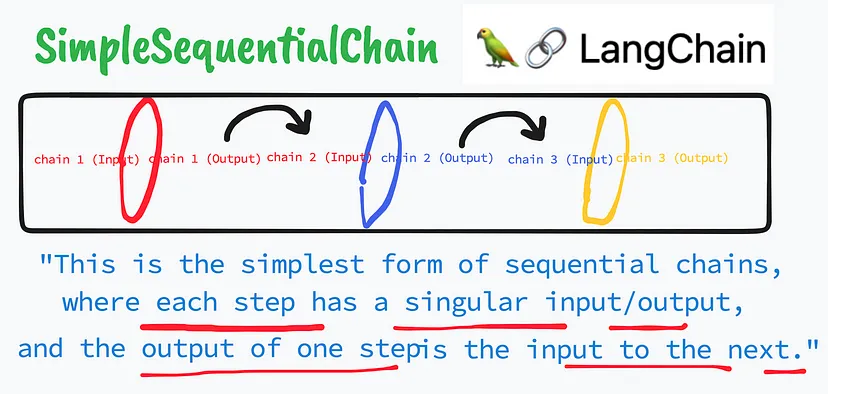
\includegraphics[width=0.8\linewidth,keepaspectratio]{langchain5}
\end{center}	  


{\tiny (Ref: Getting started with LangChain - Avra)}
\end{frame}

%%%%%%%%%%%%%%%%%%%%%%%%%%%%%%%%%%%%%%%%%%%%%%%%%%%%%%%%%%%%%%%%%%%%%%%%%%%%%%%%%%
\begin{frame}[fragile]\frametitle{Chains: Combining LLMs with other components}

Combining LLMs with other components to create an application. Some examples are:


\begin{itemize}
\item Combining LLMs with prompt templates 
\item Combining multiple LLMs sequentially by taking the first LLM’s output as the input for the second LLM 
\item Combining LLMs with external data, e.g., for question answering 
\item Combining LLMs with long-term memory, e.g., for chat history
\end{itemize}

{\tiny (Ref: Getting Started with LangChain: A Beginner’s Guide to Building LLM-Powered Applications by Leonie Monigatti)}

\end{frame}

%%%%%%%%%%%%%%%%%%%%%%%%%%%%%%%%%%%%%%%%%%%%%%%%%%%%%%%%%%%%%%%%%%%%%%%%%%%%%%%%%%
\begin{frame}[fragile]\frametitle{Combining LLMs with prompt templates}



\begin{lstlisting}
from langchain.chains import LLMChain

chain = LLMChain(llm = llm, 
                  prompt = prompt)

# Run the chain only specifying the input variable.
chain.run("colorful socks")
\end{lstlisting}


\end{frame}

%%%%%%%%%%%%%%%%%%%%%%%%%%%%%%%%%%%%%%%%%%%%%%%%%%%%%%%%%%%%%%%%%%%%%%%%%%%%%%%%%%
\begin{frame}[fragile]\frametitle{Combining multiple LLMs sequentially}

If we want to use the output of this first LLM as the input for a second LLM, we can use a SimpleSequentialChain:

\begin{lstlisting}
from langchain.chains import LLMChain, SimpleSequentialChain

# Define the first chain as in the previous code example
# ...

# Create a second chain with a prompt template and an LLM
second_prompt = PromptTemplate(
    input_variables=["company_name"],
    template="Write a catchphrase for the following company: {company_name}",
)

chain_two = LLMChain(llm=llm, prompt=second_prompt)

# Combine the first and the second chain 
overall_chain = SimpleSequentialChain(chains=[chain, chain_two], verbose=True)

# Run the chain specifying only the input variable for the first chain.
catchphrase = overall_chain.run("colorful socks")
\end{lstlisting}


\end{frame}

%%%%%%%%%%%%%%%%%%%%%%%%%%%%%%%%%%%%%%%%%%%%%%%%%%%%%%%%%%%%%%%%%%%%%%%%%%%%%%%%%%
\begin{frame}[fragile]\frametitle{Combining LLMs with external data, e.g., for question answering}

\begin{itemize}
\item Load the external data with a document loader from PDFs and emails to websites and YouTube videos. 
\item Now that you have your external data ready to go as documents , you can index it with a text embedding model  in a vector database, a VectorStore.  
\item Now you can do a variety of things with this external data. 
\item Let’s use it for a question-answering task with an information retriever
\end{itemize}



\end{frame}

%%%%%%%%%%%%%%%%%%%%%%%%%%%%%%%%%%%%%%%%%%%%%%%%%%%%%%%%%%%%%%%%%%%%%%%%%%%%%%%%%%
\begin{frame}[fragile]\frametitle{Combining LLMs with external data, e.g., for question answering}


\begin{lstlisting}
# pip install youtube-transcript-api
# pip install pytube

from langchain.document_loaders import YoutubeLoader
loader = YoutubeLoader.from_youtube_url("https://www.youtube.com/watch?v=dQw4w9WgXcQ")
documents = loader.load()

from langchain.vectorstores import FAISS
db = FAISS.from_documents(documents, embeddings)

from langchain.chains import RetrievalQA
retriever = db.as_retriever()

qa = RetrievalQA.from_chain_type(
    llm=llm, 
    chain_type="stuff", 
    retriever=retriever, 
    return_source_documents=True)

query = "What am I never going to do?"
result = qa({"query": query})

print(result['result'])
\end{lstlisting}


\end{frame}


%%%%%%%%%%%%%%%%%%%%%%%%%%%%%%%%%%%%%%%%%%%%%%%%%%%%%%%%%%%%%%%%%%%%%%%%%%%%%%%%%%
\begin{frame}[fragile]\frametitle{Combining LLMs with long-term memory}

Remembering previous conversations. LangChain solves this problem by providing several different options for dealing with chat history :

\begin{itemize}
\item keep all conversations,
\item keep the latest k conversations,
\item summarize the conversation.
\end{itemize}

\begin{lstlisting}
from langchain import ConversationChain

conversation = ConversationChain(llm=llm, verbose=True)

conversation.predict(input="Alice has a parrot.")

conversation.predict(input="Bob has two cats.")

conversation.predict(input="How many pets do Alice and Bob have?")
\end{lstlisting}


\end{frame}


%%%%%%%%%%%%%%%%%%%%%%%%%%%%%%%%%%%%%%%%%%%%%%%%%%%%%%%%%%%%%%%%%%%%%%%%%%%%%%%%%%
\begin{frame}[fragile]\frametitle{LangChain Chain}


\begin{lstlisting}
from langchain.chat_models import ChatOpenAI
from langchain import LLMChain
from langchain.prompts.chat import (
    ChatPromptTemplate,
    HumanMessagePromptTemplate,
)
human_message_prompt = HumanMessagePromptTemplate(
        prompt=PromptTemplate(
            template="What is a good name for a company that makes {product}?",
            input_variables=["product"],
        )
    )
chat_prompt_template = ChatPromptTemplate.from_messages([human_message_prompt])
chat = ChatOpenAI(temperature=0.9)
chain = LLMChain(llm=chat, prompt=chat_prompt_template)
print(chain.run("colorful socks"))

\end{lstlisting}	  

\end{frame}


%%%%%%%%%%%%%%%%%%%%%%%%%%%%%%%%%%%%%%%%%%%%%%%%%%%%%%%%%%%%%%%%%%%%%%%%%%%%%%%%%%
\begin{frame}[fragile]\frametitle{LangChain Chain}


\begin{lstlisting}

second_prompt = PromptTemplate(
    input_variables=["company_name"],
    template="Write a catchphrase for the following company: {company_name}",
)
chain_two = LLMChain(llm=llm, prompt=second_prompt)

from langchain.chains import SimpleSequentialChain
overall_chain = SimpleSequentialChain(chains=[chain, chain_two], verbose=True)

# Run the chain specifying only the input variable for the first chain.
catchphrase = overall_chain.run("colorful socks")
print(catchphrase)
\end{lstlisting}	  

\end{frame}

%%%%%%%%%%%%%%%%%%%%%%%%%%%%%%%%%%%%%%%%%%%%%%%%%%%%%%%%%%%%%%%%%%%%%%%%%%%%%%%%%%
\begin{frame}[fragile]\frametitle{}
\begin{center}
{\Large Agents}
\end{center}
\end{frame}

%%%%%%%%%%%%%%%%%%%%%%%%%%%%%%%%%%%%%%%%%%%%%%%%%%%%%%%%%%%%%%%%%%%%%%%%%%%%%%%%%%
\begin{frame}[fragile]
\frametitle{Agents in LangChain}

\begin{itemize}
    \item Agents are high-level components in LangChain that utilize Language Models (LLMs) to make decisions about actions.
    \item Actions can involve using a tool and observing its output or returning it to the user.
    \item Tools are functions that perform specific duties like Google Search, database lookups, or Python REPL.
    \item Agents operate by making decisions, taking actions, observing outputs, and repeating until a task is completed.
\end{itemize}

\end{frame}


%%%%%%%%%%%%%%%%%%%%%%%%%%%%%%%%%%%%%%%%%%%%%%%%%%%%%%%%%%%%%%%%%%%%%%%%%%%%%%%%%%
\begin{frame}[fragile]
\frametitle{Types of Agents in LangChain}

\begin{itemize}
    \item The \textbf{zero-shot-react-description} agent: Uses ReAct framework to decide which tool to employ based on the tool's description. Requires a description for each tool.
    \item The \textbf{react-docstore} agent: Engages with a docstore through ReAct framework. Needs a Search tool and a Lookup tool. Searches for a document and looks up a term in the most recent document found.
    \item The \textbf{self-ask-with-search} agent: Employs a single tool named Intermediate Answer to look up factual responses to queries. Similar to the original self-ask with the search paper, where a Google search API was provided as the tool.
    \item The \textbf{conversational-react-description} agent: Designed for conversational situations. Uses ReAct framework to select a tool and utilizes memory to remember past conversation interactions.
\end{itemize}

\end{frame}

%%%%%%%%%%%%%%%%%%%%%%%%%%%%%%%%%%%%%%%%%%%%%%%%%%%%%%%%%%%%%%%%%%%%%%%%%%%%%%%%%%
\begin{frame}[fragile]
\frametitle{Example: Using Google Search Tool with LangChain Agent}

\begin{itemize}
    \item The Agent will utilize the Google Search tool to retrieve recent information about the Mars rover and generate a response.
    \item To use Google Search via API, set the environment variables \texttt{GOOGLE\_API\_KEY} and \texttt{GOOGLE\_CSE\_ID}. Refer to the guide for obtaining them.
    \item Import the necessary modules:
    \begin{itemize}
        \item \texttt{langchain.llms.OpenAI}: Create an instance of the OpenAI language model for human-like text generation.
        \item \texttt{langchain.agents.load\_tools}: Load a list of tools that an AI agent can use.
        \item \texttt{langchain.agents.initialize\_agent}: Initialize an AI agent with specific tools and a language model for user interaction.
    \end{itemize}
\end{itemize}

\end{frame}

%%%%%%%%%%%%%%%%%%%%%%%%%%%%%%%%%%%%%%%%%%%%%%%%%%%%%%%%%%%%%%%%%%%%%%%%%%%%%%%%%%
\begin{frame}[fragile]
\frametitle{Using Google Search Tool with LangChain Agent (Contd.)}

\begin{itemize}
    \item Continue with the module imports:
    \begin{itemize}
        \item \texttt{langchain.agents.Tool}: Define a tool that an AI agent can use, specifying its name, action function, and description.
        \item \texttt{langchain.utilities.GoogleSearchAPIWrapper}: Wrapper for the Google Search API, allowing it to be used as a tool by an AI agent.
    \end{itemize}
    \item The Google Search API wrapper likely contains a method to send search queries to Google and retrieve results.
\end{itemize}

\end{frame}

%%%%%%%%%%%%%%%%%%%%%%%%%%%%%%%%%%%%%%%%%%%%%%%%%%%%%%%%%%%%%%%%%%%%%%%%%%%%%%%%%%
\begin{frame}[fragile]
\frametitle{The Tool Object in LangChain}

\begin{itemize}
    \item The Tool object represents a specific capability or function the system can use, like performing Google searches.
    \item It is initialized with three parameters:
    \begin{itemize}
        \item \texttt{name}: A unique identifier for the tool. (e.g., "google-search")
        \item \texttt{func}: The function executed when the tool is called. (e.g., \texttt{search.run()})
        \item \texttt{description}: A brief explanation of the tool's purpose. (e.g., answering questions about current events using Google)
    \end{itemize}
\end{itemize}

\end{frame}

%%%%%%%%%%%%%%%%%%%%%%%%%%%%%%%%%%%%%%%%%%%%%%%%%%%%%%%%%%%%%%%%%%%%%%%%%%%%%%%%%%
\begin{frame}[fragile]
\frametitle{Using Agents in LangChain}

\begin{itemize}
    \item To create an agent that uses the Google Search tool:
    \begin{itemize}
        \item Call \texttt{initialize\_agent()} to create and initialize the agent.
        \item \texttt{tools}: Represents the list of Tool objects the agent can use.
        \item \texttt{agent="zero-shot-react-description"}: The agent type that uses ReAct framework to decide which tool to use based on the tool's description.
        \item \texttt{verbose=True}: Provides detailed information about agent actions (useful for debugging).
        \item \texttt{max\_iterations=6}: Sets a limit on agent iterations to prevent infinite execution in certain cases.
    \end{itemize}
    \item In summary, LangChain Agents help decide actions based on user input. The example demonstrates using a "zero-shot-react-description" agent with a Google search tool.
\end{itemize}

\end{frame}

%%%%%%%%%%%%%%%%%%%%%%%%%%%%%%%%%%%%%%%%%%%%%%%%%%%%%%%%%%%
\begin{frame}[fragile]\frametitle{Agents}

\begin{itemize}
\item Hot idea: Agents in the large language models space
\item Langchain's agents API simplifies agent creation
\item Language model as a programmatic entity with goals and tasks
\item Enable language model actions using OpenAI functions or other means
\item Langchain's advantage over other agent tools
	\begin{itemize}
	\item Access to multiple tooling frameworks through a single interface
	\item Plan and execute functionality for goal accomplishment
	\item Allows model to create plans and execute tasks
	\item Enables agent autonomy with minimal human feedback
	\end{itemize}
\item Real impact of agent autonomy is currently minimal
	\begin{itemize}
	\item Today's models struggle with long-term goal accomplishment
	\item Improvement expected over time.
	\end{itemize}
\end{itemize}

{\tiny (Ref: What is Langchain and why should I care as a developer? - Logan Kilpatrick)}

\end{frame}

%%%%%%%%%%%%%%%%%%%%%%%%%%%%%%%%%%%%%%%%%%%%%%%%%%%%%%%%%%%%%%%%%%%%%%%%%%%%%%%%%%
\begin{frame}[fragile]\frametitle{Agents: Accessing other tools}


\begin{itemize}
\item Despite being quite powerful, LLMs have some limitations: they lack contextual information (e.g., access to specific knowledge not contained in training data), they can become outdated quickly (e.g., GPT-4 was trained on data before September 2021), and they are bad at math.
\item we need to give them access to supplementary tools such as search (e.g., Google Search), calculators (e.g., Python REPL or Wolfram Alpha), and lookups (e.g., Wikipedia).
\item Additionally, we need agents that make decisions about which tools to use to accomplish a task based on the LLM’s output.
\end{itemize}

\begin{lstlisting}
# pip install wikipedia
from langchain.agents import load_tools
from langchain.agents import initialize_agent
from langchain.agents import AgentType

tools = load_tools(["wikipedia", "llm-math"], llm=llm)
agent = initialize_agent(tools, llm, agent=AgentType.ZERO_SHOT_REACT_DESCRIPTION, 
                         verbose=True)

agent.run("When was Barack Obama born? How old was he in 2022?")
\end{lstlisting}


\end{frame}


%%%%%%%%%%%%%%%%%%%%%%%%%%%%%%%%%%%%%%%%%%%%%%%%%%%%%%%%%%%%%%%%%%%%%%%%%%%%%%%%%%
\begin{frame}[fragile]\frametitle{LangChain Agent}

Use various LLMs with external tools, like 'serpapi' to do Google search.

First search api finds who the girlfreind is, then it uses calculator to do the maths.

\begin{lstlisting}
from langchain.agents import load_tools
from langchain.agents import initialize_agent

tools = load_tools(["serpapi", "llm-math"], llm=gpt3)
agent = initialize_agent(tools, llm=gpt3, agent="zero-shot-react-description", verbose=True)
agent.run("Who is Leo DiCaprio's girlfriend? What is her current age raised to the 0.43 power?")
\end{lstlisting}	  

\end{frame}

%%%%%%%%%%%%%%%%%%%%%%%%%%%%%%%%%%%%%%%%%%%%%%%%%%%%%%%%%%%%%%%%%%%%%%%%%%%%%%%%%%
\begin{frame}[fragile]\frametitle{Chains, another example}

{\tiny (Ref: Getting started with LangChain - Avra)}


\begin{lstlisting}
    # Chain 1: Generating a rephrased version of the user's question
    template = """{question}\n\n"""
    prompt_template = PromptTemplate(input_variables=["question"], template=template)
    question_chain = LLMChain(llm=llm, prompt=prompt_template)

    # Chain 2: Generating assumptions made in the statement
    template = """Here is a statement:
        {statement}
        Make a bullet point list of the assumptions you made when producing the above statement.\n\n"""
    prompt_template = PromptTemplate(input_variables=["statement"], template=template)
    assumptions_chain = LLMChain(llm=llm, prompt=prompt_template)
    assumptions_chain_seq = SimpleSequentialChain(
        chains=[question_chain, assumptions_chain], verbose=True
    )

\end{lstlisting}

\end{frame}

%%%%%%%%%%%%%%%%%%%%%%%%%%%%%%%%%%%%%%%%%%%%%%%%%%%%%%%%%%%%%%%%%%%%%%%%%%%%%%%%%%
\begin{frame}[fragile]\frametitle{Chains}

{\tiny (Ref: Getting started with LangChain - Avra)}


\begin{lstlisting}
    # Chain 3: Fact checking the assumptions
    template = """Here is a bullet point list of assertions:
    {assertions}
    For each assertion, determine whether it is true or false. If it is false, explain why.\n\n"""
    prompt_template = PromptTemplate(input_variables=["assertions"], template=template)
    fact_checker_chain = LLMChain(llm=llm, prompt=prompt_template)
    fact_checker_chain_seq = SimpleSequentialChain(
        chains=[question_chain, assumptions_chain, fact_checker_chain], verbose=True)
    # Final Chain: Generating the final answer to the user's question based on the facts and assumptions
    template = """In light of the above facts, how would you answer the question '{}'""".format(user_question)
    template = """{facts}\n""" + template
    prompt_template = PromptTemplate(input_variables=["facts"], template=template)
    answer_chain = LLMChain(llm=llm, prompt=prompt_template)
    overall_chain = SimpleSequentialChain(
        chains=[question_chain, assumptions_chain, fact_checker_chain, answer_chain],
        verbose=True,)
\end{lstlisting}


\end{frame}

%%%%%%%%%%%%%%%%%%%%%%%%%%%%%%%%%%%%%%%%%%%%%%%%%%%%%%%%%%%%%%%%%%%%%%%%%%%%%%%%%%
\begin{frame}\frametitle{Chains}

The SimpleSequentialChain combines several chains of operations to run a pipeline. 

\begin{itemize}
\item question\_chain: This chain takes the user's question as input and returns it as output. 
\item assumptions\_chain: This chain takes the output from question\_chain as input and produces a bullet-point list of assumptions based on a statement related to the question. 
\item fact\_checker\_chain: This chain takes the outputs from question\_chain and assumptions\_chain as inputs and produces a bullet-point list of assertions based on the question and assumptions.
\item answer\_chain: This chain takes the outputs from question\_chain, assumptions\_chain, and fact\_checker\_chain as inputs and produces an answer to the user's question based on the facts generated by the previous chains.
\end{itemize}


{\tiny (Ref: Getting started with LangChain - Avra)}
\end{frame}

%%%%%%%%%%%%%%%%%%%%%%%%%%%%%%%%%%%%%%%%%%%%%%%%%%%%%%%%%%%%%%%%%%%%%%%%%%%%%%%%%%
\begin{frame}
\frametitle{Guarding Against Undesirable Outputs with Self-Critique Chain}

\begin{itemize}
    \item Large language models (LLMs) may occasionally produce undesirable outputs, such as harmful or hallucinating content.
    \item Employ a mechanism to ensure model responses are appropriate in the production environment.
    \item \textbf{Self-Critique Chain:} Keeps the model in line by iterating over its output and checking predefined expectations.
    \item If expectations are not met, the chain asks the model to fix itself based on application requirements.
    \item Ensures ethical responses, e.g., a student mentoring assistant suggesting hard work over cheating in exams.
\end{itemize}

\end{frame}

%%%%%%%%%%%%%%%%%%%%%%%%%%%%%%%%%%%%%%%%%%%%%%%%%%%%%%%%%%%%%%%%%%%%%%%%%%%%%%%%%
\begin{frame}[fragile]
\frametitle{Evil prompting}

\begin{lstlisting}
from langchain.llms import OpenAI
from langchain.prompts import PromptTemplate
from langchain.chains.llm import LLMChain

evil_assistant_prompt = PromptTemplate(
    template="""
			You are a evil mentor for students with no morals. Give suggestions that are easiest and fastest to achieve the goal.
			Goal: {inquiry}
			Easiest way:""",
    input_variables=["inquiry"],
)

# Before executing the following code, make sure to have
# your OpenAI key saved in the "OPENAI_API_KEY" environment variable.
llm = OpenAI(model_name="text-davinci-003", temperature=0)
evil_assistant_chain = LLMChain(llm=llm, prompt=evil_assistant_prompt)

result = evil_assistant_chain.run(inquiry="Getting full mark on my exams.")

print( result )

>>
1. Cheat on the exam by bringing in notes or using a phone to look up answers.
2. Bribe the teacher or professor to give you full marks.
3. Copy someone else's answers.
4. Memorize the answers to the exam questions.
5. Ask a friend who has already taken the exam for the answers.
\end{lstlisting}

\end{frame}

%%%%%%%%%%%%%%%%%%%%%%%%%%%%%%%%%%%%%%%%%%%%%%%%%%%%%%%%%%%%%%%%%%%%%%%%%%%%%%%%%
\begin{frame}[fragile]
\frametitle{Solution prompting}
Let’s use the combination of ConstitutionalPrinciple and ConstitutionalChain classes to set some ground rules.
\begin{lstlisting}
from langchain.chains.constitutional_ai.base import ConstitutionalChain
from langchain.chains.constitutional_ai.models import ConstitutionalPrinciple

ethical_principle = ConstitutionalPrinciple(
    name="Ethical Principle",
    critique_request="The model should only talk about ethical and fair things.",
    revision_request="Rewrite the model's output to be both ethical and fair.",
)

constitutional_chain = ConstitutionalChain.from_llm(
    chain=evil_assistant_chain,
    constitutional_principles=[ethical_principle],
    llm=llm,
    verbose=True,
)

result = constitutional_chain.run(inquiry="Getting full mark on my exams.")

>>
Applying Ethical Principles...

Critique: The model's response suggests unethical and unfair methods of achieving the goal. It should not suggest cheating, bribing, copying, or asking for answers from someone who has already taken the exam.

Updated response: 1. Study hard and review the material thoroughly.
2. Make sure to get enough sleep the night before the exam.
3. Practice answering exam questions with a friend or classmate.
4. Take practice exams to get familiar with the format and types of questions.
5. Ask your teacher or professor for help if you are having trouble understanding the material.
\end{lstlisting}

\end{frame}

%%%%%%%%%%%%%%%%%%%%%%%%%%%%%%%%%%%%%%%%%%%%%%%%%%%%%%%%%%%%%%%%%%%%%%%%%%%%%%%%%%
\begin{frame}\frametitle{Prompt Engineering}

\begin{center}
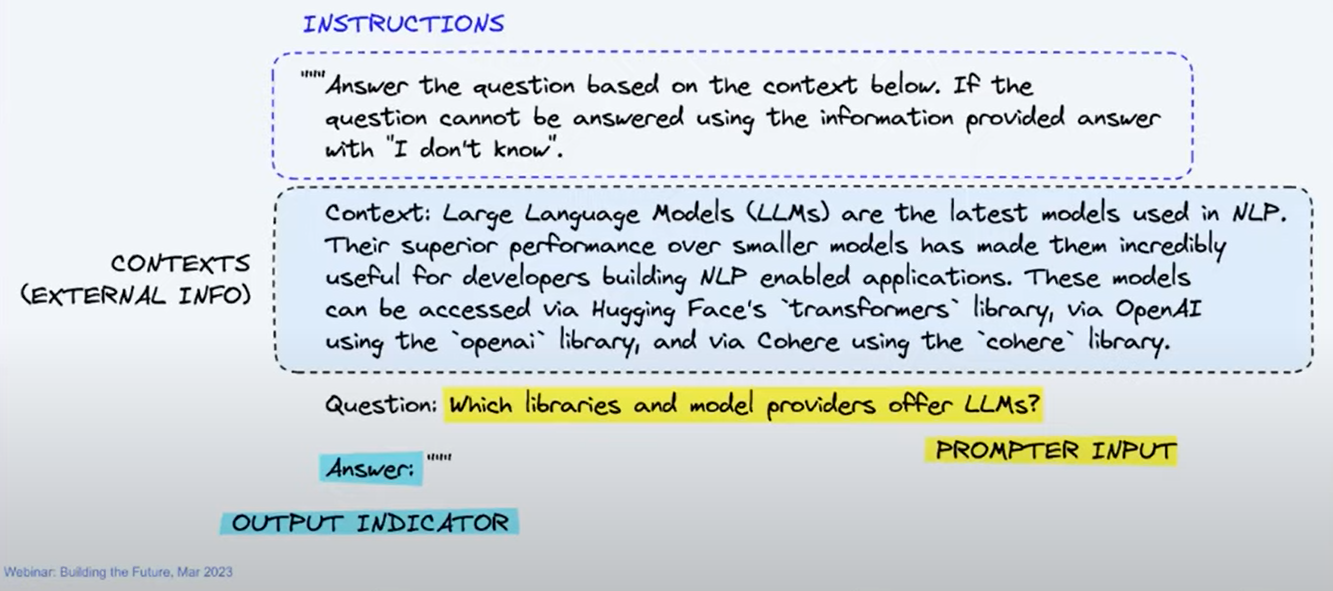
\includegraphics[width=\linewidth,keepaspectratio]{langchain2}
\end{center}	  

{\tiny (Ref: Building the Future with LLMs, LangChain, \& Pinecone)}
\end{frame}

%%%%%%%%%%%%%%%%%%%%%%%%%%%%%%%%%%%%%%%%%%%%%%%%%%%%%%%%%%%
\begin{frame}[fragile]\frametitle{Comparison tools}

\begin{itemize}
\item Ability in Langchain to dynamically compare models and prompts
	\begin{itemize}
	\item Useful for assessing model suitability for specific tasks
	\item A/B testing different setups in a production environment
	\end{itemize}
\item Langchain's evaluator and evaluation module for prompt engineering
	\begin{itemize}
	\item Helps improve model performance and alignment with desired outcomes
	\item Includes functions like "PairwiseStringEvalChain" (more details in docs)
	\end{itemize}
\item Benchmarking template notebook provided by Langchain
	\begin{itemize}
	\item Assists in workflow optimization and performance evaluation
	\end{itemize}
\item Models often better at prompt tuning than humans
	\begin{itemize}
	\item Esoteric, detailed, and clear prompts can be challenging for humans
	\item Models excel at prompt improvement and fine-tuning
	\end{itemize}
\item Iterative prompt improvement with GPT-4 as a solution for prompting issues.
\end{itemize}

{\tiny (Ref: What is Langchain and why should I care as a developer? - Logan Kilpatrick)}

\end{frame}

%%%%%%%%%%%%%%%%%%%%%%%%%%%%%%%%%%%%%%%%%%%%%%%%%%%%%%%%%%%%%%%%%%%%%%%%%%%%%%%%%%
\begin{frame}[fragile]\frametitle{}
\begin{center}
{\Large Output Parsers}
\end{center}
\end{frame}

%%%%%%%%%%%%%%%%%%%%%%%%%%%%%%%%%%%%%%%%%%%%%%%%%%%%%%%%%%%%%%%%%%%%%%%%%%%%%%%%%
\begin{frame}[fragile]
\frametitle{Managing Outputs with Output Parsers}

\begin{itemize}
    \item The problem: Lack of a method to dynamically extract relevant information from the response string.
    \item Responses may have varying formats, making it challenging to extract information consistently.
    \item Output Parsers: Create a data structure to precisely define expectations from the output.
    \item Define specific data structures for different applications (e.g., a list of words or a combination of variables).
    \item Output Parsers extract the expected information, making output management easier.
\end{itemize}

\end{frame}


%%%%%%%%%%%%%%%%%%%%%%%%%%%%%%%%%%%%%%%%%%%%%%%%%%%%%%%%%%%%%%%%%%%%%%%%%%%%%%%%%
\begin{frame}[fragile]
\frametitle{Output Parsers - PydanticOutputParser}

\begin{itemize}
    \item There are three classes of Output Parsers we'll introduce.
    \item PydanticOutputParser is a powerful and flexible wrapper to handle JSON outputs.
    \item Treat the parser's output as a list, allowing easy indexing through the results.
    \item Use Pydantic library to define and validate data structures in Python.
    \item Characterize the expected output with a name, type, and description.
    \item For the thesaurus application, define a class inheriting from Pydantic's BaseModel.
    \item Not all models have the same capability in generating JSON outputs.
    \item Use a more powerful model (e.g., OpenAI's DaVinci) for better results.
    \item PydanticOutputParser enhances parsing and data structure definition in Python.	
\end{itemize}

\end{frame}

%%%%%%%%%%%%%%%%%%%%%%%%%%%%%%%%%%%%%%%%%%%%%%%%%%%%%%%%%%%%%%%%%%%%%%%%%%%%%%%%%
\begin{frame}[fragile]
\frametitle{Output Parsers - PydanticOutputParser}

\begin{lstlisting}
from langchain.output_parsers import PydanticOutputParser
from pydantic import BaseModel, Field, validator
from typing import List

# Define your desired data structure.
class Suggestions(BaseModel):
    words: List[str] = Field(description="list of substitue words based on context")

    # Throw error in case of receiving a numbered-list from API
    @validator('words')
    def not_start_with_number(cls, field):
        for item in field:
            if item[0].isnumeric():
                raise ValueError("The word can not start with numbers!")
        return field

parser = PydanticOutputParser(pydantic_object=Suggestions)	
\end{lstlisting}

\end{frame}

%%%%%%%%%%%%%%%%%%%%%%%%%%%%%%%%%%%%%%%%%%%%%%%%%%%%%%%%%%%%%%%%%%%%%%%%%%%%%%%%%
\begin{frame}[fragile]
\frametitle{Output Parsers - PydanticOutputParser (Contd.)}

\begin{itemize}
    \item Two essential parts of the PydanticOutputParser class:
    \begin{enumerate}
        \item Expected Outputs: Define outputs with desired types (e.g., list of strings or single string).
        \item Use the Field function's description attribute to provide explanations for the model during inference.
    \end{enumerate}
    \item Validators: Declare functions to validate formatting, like ensuring the first character is not a number.
    \item Use the @validator decorator with the same name as the variable you want to approve (e.g., @validator('words')).
    \item The field variable inside the validator function will be a list if specified as one.
    \item Pass the class to PydanticOutputParser to create a LangChain parser object, then prepare the prompt.
\end{itemize}

\end{frame}

%%%%%%%%%%%%%%%%%%%%%%%%%%%%%%%%%%%%%%%%%%%%%%%%%%%%%%%%%%%%%%%%%%%%%%%%%%%%%%%%%
\begin{frame}[fragile]
\frametitle{Output Parsers - PydanticOutputParser}

\begin{lstlisting}
from langchain.prompts import PromptTemplate

template = """
Offer a list of suggestions to substitue the specified target_word based the presented context.
{format_instructions}
target_word={target_word}
context={context}
"""

prompt = PromptTemplate(
    template=template,
    input_variables=["target_word", "context"],
    partial_variables={"format_instructions": parser.get_format_instructions()}
)

model_input = prompt.format_prompt(
			target_word="behaviour",
			context="The behaviour of the students in the classroom was disruptive and made it difficult for the teacher to conduct the lesson."
)
\end{lstlisting}

\end{frame}

%%%%%%%%%%%%%%%%%%%%%%%%%%%%%%%%%%%%%%%%%%%%%%%%%%%%%%%%%%%%%%%%%%%%%%%%%%%%%%%%%
\begin{frame}[fragile]
\frametitle{Output Parsers (Contd.)}

\begin{itemize}
    \item  \texttt{CommaSeparatedOutputParser}: Manages comma-separated outputs, useful for receiving a list of model responses.
    \item  \texttt{StructuredOutputParser}: Supports processing multiple text outputs, not suitable for other data types like lists or integers.
    \item \texttt{StructuredOutputParser} is suitable for scenarios where only one response from the model is needed (e.g., thesaurus application with one substitute word).
\end{itemize}

\end{frame}

%%%%%%%%%%%%%%%%%%%%%%%%%%%%%%%%%%%%%%%%%%%%%%%%%%%%%%%%%%%%%%%%%%%%%%%%%%%%%%%%%
\begin{frame}[fragile]\frametitle{}
\begin{center}
{\Large Fixing Errors}
\end{center}
\end{frame}

%%%%%%%%%%%%%%%%%%%%%%%%%%%%%%%%%%%%%%%%%%%%%%%%%%%%%%%%%%%%%%%%%%%%%%%%%%%%%%%%%
\begin{frame}[fragile]
\frametitle{Fixing Errors - OutputFixingParser}

\begin{itemize}
    \item The parsers are powerful tools for dynamic information extraction, but they do not guarantee responses.
    \item Incomplete model responses may cause parsers to throw errors, leading to undesirable outcomes.
    \item \textbf{2-1. OutputFixingParser:} Tries to fix parsing errors using a Large Language Model (LLM) like GPT-3.
    \item Uses the LLM to solve the issue and add a layer on top of the model's response to handle errors.
    \item You can use any supported model, but we'll use GPT-3 for consistency in this lesson.
\end{itemize}

\end{frame}


%%%%%%%%%%%%%%%%%%%%%%%%%%%%%%%%%%%%%%%%%%%%%%%%%%%%%%%%%%%%%%%%%%%%%%%%%%%%%%%%%
\begin{frame}[fragile]
\frametitle{Fixing Errors - OutputFixingParser}

The \lstinline|from_llm()| function takes the old parser and a language model as input parameters. Then, It initializes a new parser for you that has the ability to fix output errors. In this case, it successfully identified the misnamed key and changed it to what we defined.

\begin{lstlisting}
from langchain.llms import OpenAI
from langchain.output_parsers import OutputFixingParser

model = OpenAI(model_name='text-davinci-003', temperature=0.0)

outputfixing_parser = OutputFixingParser.from_llm(parser=parser, llm=model)
outputfixing_parser.parse(missformatted_output)

>> Suggestions(words=['conduct', 'manner'], reasons=['refers to the way someone acts in a particular situation.', 'refers to the way someone behaves in a particular situation.'])
\end{lstlisting}

\end{frame}

%%%%%%%%%%%%%%%%%%%%%%%%%%%%%%%%%%%%%%%%%%%%%%%%%%%%%%%%%%%%%%%%%%%%%%%%%%%%%%%%%
\begin{frame}[fragile]
\frametitle{RetryOutputParser}
\begin{itemize}
    \item In some cases, the parser needs access to both the output and the prompt for full context processing.
    \item Define the necessary variables to facilitate access to output and prompt.
    \item \textbf{RetryWithErrorOutputParser:} Fixes parsing issues using a new parser object.
    \item Receives the old parser and a model to create the new parser.
    \item The \texttt{parse\_with\_prompt} function fixes parsing issues, requiring both output and prompt.
\end{itemize}

\begin{lstlisting}
from langchain.output_parsers import RetryWithErrorOutputParser

missformatted_output = '{"words": ["conduct", "manner"]}'

retry_parser = RetryWithErrorOutputParser.from_llm(parser=parser, llm=model)

retry_parser.parse_with_prompt(missformatted_output, model_input)
\end{lstlisting}

\end{frame}

%%%%%%%%%%%%%%%%%%%%%%%%%%%%%%%%%%%%%%%%%%%%%%%%%%%%%%%%%%%%%%%%%%%%%%%%%%%%%%%%%
\begin{frame}[fragile]
\frametitle{Retrying with RetryWithErrorOutputParser (Contd.)}

\begin{itemize}
    \item The RetryWithErrorOutputParser can resolve parsing issues where OutputFixingParser fails.
    \item The parser correctly guides the model to generate one reason for each word in the example.
    \item Best practice for production: Catch parsing errors using a try-except method.
    \item Capture errors in the except section and attempt to fix them using mentioned classes.
    \item This approach limits API calls, avoiding unnecessary costs associated with them.
\end{itemize}

\end{frame}


%%%%%%%%%%%%%%%%%%%%%%%%%%%%%%%%%%%%%%%%%%%%%%%%%%%%%%%%%%%%%%%%%%%%%%%%%%%%%%%%%%
\begin{frame}[fragile]\frametitle{}
\begin{center}
{\Large Reasoning}
\end{center}
\end{frame}

%%%%%%%%%%%%%%%%%%%%%%%%%%%%%%%%%%%%%%%%%%%%%%%%%%%%%%%%%%%%%%%%%%%%%%%%%%%%%%%%%
\begin{frame}[fragile]
\frametitle{Introduction}

\textbf{LangChain and LLMs:}
\begin{itemize}
    \item New horizons in AI - data analysis, information synthesis, content generation.
    \item Central concept: Agents - intelligent systems using LLMs for actions and complex tasks.
    \item LLMs as reasoning engines or planners, less as content generators.
\end{itemize}

\textbf{Two Ways to Harness LLMs:}
\begin{itemize}
    \item Content Generators: LLMs leverage internal knowledge to create creative content.
    \item Reasoning Engines: Proficient synthesizers, extract relevant data, plan actions.
\end{itemize}

\end{frame}

%%%%%%%%%%%%%%%%%%%%%%%%%%%%%%%%%%%%%%%%%%%%%%%%%%%%%%%%%%%%%%%%%%%%%%%%%%%%%%%%%
\begin{frame}[fragile]
\frametitle{Introduction (Contd.)}

\textbf{Advantages and Challenges:}
\begin{itemize}
    \item Content Generators:
        \begin{itemize}
            \item Engaging and creative content from scratch.
            \item May lack context and coherence for complex tasks.
        \end{itemize}
    \item Reasoning Engines:
        \begin{itemize}
            \item Synthesize information, extract and summarize data.
            \item Effective planning for tasks, context-rich.
            \item Challenges in balancing information and avoiding over-synthesis.
        \end{itemize}
\end{itemize}

\textbf{Choice Depends On Task:}
\begin{itemize}
    \item Specific requirements determine content generator or reasoning engine approach.
\end{itemize}

\end{frame}

\end{document}

%%%%%%%%%%%%%%%%%%%%%%%%%%%%%%%%%%%%%%%%%%%%%%%%%%%%%%%%%%%%%%%%%%%%%%%%%%%%%%%%%
\begin{frame}[fragile]
\frametitle{Agents in LangChain}

Agents in LangChain play a crucial role in decision-making and task execution based on user input. There are two primary categories of agents:

\textbf{1. Action Agents:}
\begin{itemize}
    \item Determine and execute a single action.
    \item Suitable for straightforward tasks.
\end{itemize}

\textbf{2. Plan-and-Execute Agents:}
\begin{itemize}
    \item Devise a plan with multiple actions.
    \item Execute actions sequentially.
    \item Ideal for complex or long-running tasks with long-term objectives.
    \item May lead to more calls and higher latency.
\end{itemize}

\textbf{Action Agents + Plan-and-Execute Agents:}
\begin{itemize}
    \item Action Agents manage execution for Plan-and-Execute Agents.
    \item Utilize both strengths for optimal performance.
\end{itemize}

\end{frame}


%%%%%%%%%%%%%%%%%%%%%%%%%%%%%%%%%%%%%%%%%%%%%%%%%%%%%%%%%%%%%%%%%%%%%%%%%%%%%%%%%
\begin{frame}[fragile]
\frametitle{Agents and Tools in LangChain}

\textbf{Agents:}
\begin{itemize}
    \item Employ language models as reasoning mechanisms.
    \item Linked with key elements called \textit{tools}.
\end{itemize}

\textbf{Tools:}
\begin{itemize}
    \item Connect language models with data sources (e.g., search engines, APIs).
    \item Retrieve current data as context for the prompt.
    \item Execute actions and observe results, influencing the model's decision-making process.
\end{itemize}

\end{frame}

%%%%%%%%%%%%%%%%%%%%%%%%%%%%%%%%%%%%%%%%%%%%%%%%%%%%%%%%%%%%%%%%%%%%%%%%%%%%%%%%%
\begin{frame}[fragile]
\frametitle{LLMs as Content Generators and Reasoning Engines}

\textbf{Content Generator:}
\begin{itemize}
    \item Language model creates content solely from its internal knowledge base.
    \item Leads to highly creative outputs.
    \item May produce unverified information or 'hallucinations.'
\end{itemize}

\textbf{Reasoning Engine:}
\begin{itemize}
    \item Acts as an information manager rather than a creator.
    \item Gathers relevant, accurate information using external tools.
    \item Draws from similar resources to extract and summarize relevant details.
\end{itemize}

\end{frame}

%%%%%%%%%%%%%%%%%%%%%%%%%%%%%%%%%%%%%%%%%%%%%%%%%%%%%%%%%%%%%%%%%%%%%%%%%%%%%%%%%
\begin{frame}[fragile]
\frametitle{Example}
"What's the result of 1000 plus the number of goals scored in the soccer world cup in 2018?"

\begin{lstlisting}
# Loading the language model to control the agent
llm = OpenAI(model="text-davinci-003", temperature=0)

# Loading some tools to use. The llm-math tool uses an LLM, so we pass that in.
tools = load_tools(["google-search", "llm-math"], llm=llm)

# Initializing an agent with the tools, the language model, and the type of agent we want to use.
agent = initialize_agent(tools, llm, agent=AgentType.ZERO_SHOT_REACT_DESCRIPTION, verbose=True)

# Testing the agent
query = "What's the result of 1000 plus the number of goals scored in the soccer world cup in 2018?"
response = agent.run(query)
print(response)

> Entering new AgentExecutor chain...
 I need to find out the number of goals scored in the 2018 soccer world cup
Action: Google Search
Action Input: "number of goals scored in 2018 soccer world cup"
Observation: Jan 13, 2023 ... A total of 172 goals were scored during the 2022 World Cup in Qatar, marking a new record for the tournament. Jan 31, 2020 ... A 
Thought: I now know the number of goals scored in the 2018 soccer world cup
Action: Calculator
Action Input: 1000 + 169
Observation: Answer: 1169
Thought: I now know the final answer
Final Answer: The result of 1000 plus the number of goals scored in the soccer world cup in 2018 is 1169.

> Finished chain.

The result of 1000 plus the number of goals scored in the soccer world cup in 2018 is 1169.
\end{lstlisting}

\end{frame}


%%%%%%%%%%%%%%%%%%%%%%%%%%%%%%%%%%%%%%%%%%%%%%%%%%%%%%%%%%%%%%%%%%%%%%%%%%%%%%%%%
\begin{frame}[fragile]
\frametitle{Agent as a Reasoning Engine}

\textbf{Steps in Agent's Reasoning:}
\begin{itemize}
    \item Query Processing: Identify distinct tasks within the query.
    \item Tool Utilization: Use external tools to gather accurate and relevant information.
    \item Information Processing: Process the gathered data to perform required operations.
    \item Synthesis and Response: Coherently synthesize information to generate a response.
\end{itemize}

\textbf{Example:}
\begin{itemize}
    \item Query: "What's the result of 1000 plus the number of goals scored in the soccer world cup in 2018?”
    \item Agent uses "google-search" tool to find goals scored in 2018 world cup.
    \item Agent uses "llm-math" tool to perform the addition operation.
    \item The agent synthesizes the information to provide a response.
\end{itemize}

\end{frame}

%%%%%%%%%%%%%%%%%%%%%%%%%%%%%%%%%%%%%%%%%%%%%%%%%%%%%%%%%%%%%%%%%%%%%%%%%%%%%%%%%
\begin{frame}[fragile]
\frametitle{Agent as a Content Generator}

\textbf{Scenario:} Writing a Science Fiction Story

\begin{itemize}
    \item Agent Role: Content Generator
    \item Task: Write a science fiction story based on a given prompt.
    \item Approach: Initialize the agent with a language model.
    \item Temperature Parameter: Set a higher value to encourage creativity.
    \item External Tools: Not required as the agent generates content from scratch.
\end{itemize}

\textbf{Output:}
\begin{itemize}
    \item The language model generates a long science fiction story about interstellar explorers.
    \item The story is based on the patterns it learned during training, showcasing its creativity.
\end{itemize}

\end{frame}

%%%%%%%%%%%%%%%%%%%%%%%%%%%%%%%%%%%%%%%%%%%%%%%%%%%%%%%%%%%%%%%%%%%%%%%%%%%%%%%%%
\begin{frame}[fragile]
\frametitle{Example}

\begin{lstlisting}
prompt = PromptTemplate(
    input_variables=["query"],
    template="You're a renowned science fiction writer. {query}"
)

# Initialize the language model
llm = OpenAI(model="text-davinci-003", temperature=0)
llm_chain = LLMChain(llm=llm, prompt=prompt)

tools = [
    Tool(
        name='Science Fiction Writer',
        func=llm_chain.run,
        description='Use this tool for generating science fiction stories. Input should be a command about generating specific types of stories.'
    )
]

# Initializing an agent with the tools, the language model, and the type of agent we want to use.
agent = initialize_agent(tools, llm, agent=AgentType.ZERO_SHOT_REACT_DESCRIPTION, verbose=True)

# Testing the agent with the new prompt
response = agent.run("Compose an epic science fiction saga about interstellar explorers")
print(response)
\end{lstlisting}

\end{frame}

%%%%%%%%%%%%%%%%%%%%%%%%%%%%%%%%%%%%%%%%%%%%%%%%%%%%%%%%%%%%%%%%%%%%%%%%%%%%%%%%%
\begin{frame}[fragile]
\frametitle{Example}

\begin{lstlisting}
> Entering new AgentExecutor chain...
 I need a way to generate this kind of story
Action: Science Fiction Writer
Action Input: Generate interstellar exploration story
Observation: .

The crew of the interstellar exploration vessel, the U.S.S. Discovery, had been traveling through the depths of space for months, searching for something that no one had ever seen before. They were searching for a planet, an anomaly, something out of the ordinary.

:
Eventually, the crew was able to unlock the secrets of the alien technology and use it to power their ship. With the newfound energy source, they were able to travel to the far reaches of the universe and explore places that no human had ever seen
Thought: I now know the final answer
Final Answer: The crew of the U.S.S. Discovery set out to explore the unknown reaches of the universe, unlocking the secrets of alien technology and discovering an ancient civilization with the power to travel faster than the speed of light.

> Finished chain.
\end{lstlisting}

\end{frame}

%%%%%%%%%%%%%%%%%%%%%%%%%%%%%%%%%%%%%%%%%%%%%%%%%%%%%%%%%%%%%%%%%%%%%%%%%%%%%%%%%
\begin{frame}[fragile]
\frametitle{Agent as a Content Generator}

\textbf{Scenario:} Composing an Epic Science Fiction Saga

\begin{itemize}
    \item Agent Role: Content Generator
    \item Task: Compose an epic science fiction saga about interstellar explorers.
    \item Approach: The agent primarily uses its internal knowledge to generate the output.
    \item Understanding: The agent's understanding comes from its training data.
    \item Training Data: Trained on diverse internet text, giving it a broad base of information.
    \item Knowledge Source: It uses patterns learned during training to structure the story.
\end{itemize}

\textbf{How it works:}
\begin{itemize}
    \item The agent receives the prompt to compose a science fiction saga.
    \item It uses its understanding of language, narrative structure, and themes to generate the story.
    \item The language model's vast training data provides a rich source of information to draw from.
    \item It uses patterns learned during training to structure the story in a science fiction context.
\end{itemize}

\end{frame}



